\documentclass[landscape, 8pt]{extarticle}
% \usepackage{showframe}

\usepackage[dvipsnames]{xcolor}
% custom colour definitions
\colorlet{colour1}{Red}
\colorlet{colour2}{Green}
\colorlet{colour3}{Cerulean}

\usepackage{geometry}
% margins
\geometry{
    a4paper, 
    margin=0.17in
}

\usepackage{graphicx} % Required for inserting images
\usepackage{amsmath}
\usepackage{amsfonts}
\usepackage{amssymb}
\usepackage{preamble}
\usepackage{multicol}
\usepackage{microtype}
\usepackage{stmaryrd}
\usepackage{lipsum}
\usepackage{float}
\usepackage{wrapfig}
\usepackage[nodisplayskipstretch]{setspace}


% tikz and theorem boxes
\usepackage[framemethod=TikZ]{mdframed}
\usepackage{../thmboxes_col}
% \usepackage{../thmboxes_col}



% Custom Definitions of operators
\DeclareMathOperator{\Ima}{im}
\DeclareMathOperator{\Fix}{Fix}
\DeclareMathOperator{\Orb}{Orb}
\DeclareMathOperator{\Stab}{Stab}
\DeclareMathOperator{\send}{send}
\DeclareMathOperator{\dom}{dom}

\begin{document}

% vertical gap between full length math mode equations
\setlength{\abovedisplayskip}{3.5pt}
\setlength{\belowdisplayskip}{3.5pt}
\setlength{\abovedisplayshortskip}{3.5pt}
\setlength{\belowdisplayshortskip}{3.5pt}

\begin{multicols}{3}
\raggedcolumns % don't force squeeze width of columns
\section{\huge Leon's (WIP) ITCS Exam Notes}
\vspace{-5pt}
Basically adapted from Chris Dalziel's notes :)\newline
In collaboration with Alex Brodbelt :)
\subsection*{Finite Automata}

\begin{dfn}[Finite Automata]{def:finite-Automata}{}
A finite automaton takes a string as input and replies "yes" or "no". If an automaton $A$ replies "yes" on a string $S$ we say that $A$ "accepts" $S$.
\end{dfn}

\begin{dfn}[Deterministic Finite Automata]{def:DFAs}{}

    A deterministic finite automaton (DFA) is a quintuple\newline $(Q,\Sigma, q_{0}, \delta, F)$ where
    \renewcommand\labelitemi{\tiny$\bullet$}
    \begin{itemize}
        \setlength\itemsep{0em}
        \item $Q$ is a finite set of states
        \item $\Sigma$ is an alphabet
        \item $q_{0}\in Q$ is the initial state
        \item $\delta:Q \times \Sigma \to Q$ is the transition function
        \item $F \subseteq Q$ is the set of final states
    \end{itemize}
    A DFA accepts a string $w\in \Sigma^{*}$ iff $\delta^{*}(q_{0}, w)\in F$, where $\delta^{*}$ is $\delta$ applied successively for each symbol in $w$.
    \newline
    The language of a DFA $A$ is the set of all strings accepted by $a$, $\mathcal{L}\subseteq \Sigma^{*}$ is the set of all strings accepted by $A$.
    \newline
    The transition function is a total function which gives exactly one next state for each input symbol, i.e. it is deterministic
% \begin{figure}[H]
%     \centering
%     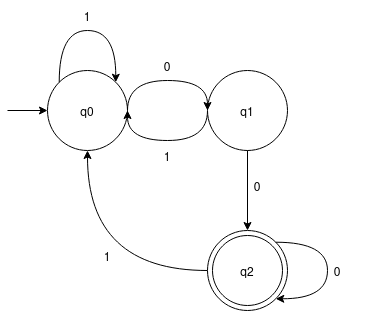
\includegraphics[width=\linewidth]{images/dfa.png}
%     \caption{Example of a DFA}
% \end{figure}
\end{dfn}


\begin{dfn}[Nondeterministic Finite Automata]{def:NDAs}{}
    Non-determinism would mean that $\delta$ can return more than one successor state, it instead returns a set of possible states - no states is an empty set. A NFA is a quintuple $(Q, \Sigma, q_0, \delta, F)$ where:
    \begin{itemize}
        \item $Q$ is a finite set of states
        \item $\Sigma$ is an alphabet
        \item $q_0 \in Q$ is the initial state
        \item $\delta : Q \times \Sigma \to \mathcal{P}(Q)$ is the transition function
        \item $F \subseteq Q$ is the set of final states
    \end{itemize}

    The only difference between the definition of a DFA and that of an NFA is that in an NFA $\delta$ returns an element from the powerset of $Q$, $\mathcal{P}(Q)$

    Adding non-determinism doesn't change "expressivity". Given an NFA $A$ there is an equivalent DFA $D$ such that $\mathcal{L}(D)=\mathcal{L}(A)$ and vice versa.

\end{dfn}

\begin{dfn}[$\epsilon$-NFA]{def:epsilon-nfas}{}
If we allow non-deterministic state chnages that don't consume any input symbols, we can label silent moves using $\epsilon$ - meaning the empty string
We define the $\epsilon$ closure $E(q)$ of a state $q$ as the set of all states reachable from $q$ by silent moves. That is, $E(q)$ is the least set satisfying:
\renewcommand\labelitemi{\tiny$\bullet$}
\begin{itemize}
    \setlength\itemsep{0em}
    \item $q\in E(q)$
    \item For any $s\in E(q)$ we also have $\delta(s, \epsilon)\subseteq E(q)$
\end{itemize}
DFA, NFA, $\epsilon$-NFA are all equal in expressive power
\end{dfn}

\subsection*{Regular Languages}
\begin{dfn}[Regular Languages]{def:reglangs}{}
Any language which can be accepted by a finite automaton is called a regular language. \newline
Regular languages are also those recognised by Regular Expressions
\end{dfn}

\begin{dfn}[Regular Language Closure Properties]{def:regex-properties}{}
    For two languages $L_{1}$ and $L_{2}$, the following operations satisfy the closure property, i.e. for a member $x\in X$, and an operation $\phi$ we have that $\phi(x)\in\mathbb{R}$ for all $x$.
    \renewcommand\labelitemi{\tiny$\bullet$}
    \begin{itemize}
        \setlength\itemsep{0em}
        \item \textbf{Union}: $L_{1}\cup L_{2}$ is the language that includes all strings of $L_{1}$ and all strings of $L_{2}$. 
        \item \textbf{Intersection}: $L_{1}\cap L_{2}$ is the language that includes all strings of $L_{1}$ that are not in $L_{2}$, and vice versa
        \item \textbf{Sequential Composition}: $L_{1}L_{2}$ is the language of strings that consist of strings in $L_{1}$ followed by a string in $L_{2}$.
        \item \textbf{Kleene closure}: $L^{*}$ is the language of strings that consist wholly of zero or more strings in $L$.
        \[L^{*} = \bigcup_{i\in\mathbb{N}} L^{i}\]
        \item \textbf{Complement}: $\bar{L}$ is the language of every string not in $L$.
    \end{itemize}
\end{dfn}


\begin{dfn}[Regular Expressions]{def:regexs}{}
Regular characterise the regular languages, just like finite automata do.
The following table shows the syntax and semantics of a regex.

\begin{table}[H]
    \begin{tabular}{l|ll}
    Syntax & Semantics                                                                                       &                  \\ \hline
    $a$             & $\llbracket a \rrbracket = \{a\}$                                                               & $(a \in \Sigma)$ \\
    $\emptyset$     & $\llbracket \emptyset \rrbracket = \emptyset$                                                   &                  \\
    $\epsilon$      & $\llbracket \epsilon \rrbracket = \{\epsilon\}$                                                 &                  \\
    $R_1 \cup R_2$  & $\llbracket R_1 \cup R_2 \rrbracket = \llbracket R_1 \rrbracket \cup \llbracket R_2 \rrbracket$ &                  \\
    $R_1 \circ R_2$ & $\llbracket R_1 \circ R_2 \rrbracket = \llbracket R_1 \rrbracket \llbracket R_2 \rrbracket$     &                  \\
    $R^*$           & $\llbracket R^* \rrbracket = \llbracket R \rrbracket^*$                                         &                 
    \end{tabular}
    \centering
\end{table}


\end{dfn}


\begin{dfn}[Generalised NFAs]{def:gnfa}{}
A \textbf{generalised NFA}, or GNFA is an NFA where:
\renewcommand\labelitemi{\tiny$\bullet$}
\begin{itemize}
    \setlength\itemsep{0em}
    \item Transitions have \textbf{regular expressions} on them instead of symbols
    \item There is only one unique final state
    \item The transition relation if \textbf{full}, except that the initial state has no incoming transitions, and the final state has no outgoing transitions
\end{itemize}
\end{dfn}

% TODO: maybe add converting DFA to GNFA

\begin{thm}[Pumping Lemma]{thm:pumping-lemma}{}
If $L\subseteq \Sigma^{*}$ is regular, then there is a \textbf{pumping length} $p\in\mathbb{N}$ such that for any $w\in L$ where $\lvert w\rvert \ge p$, we may split $w$ into three piexes $w=xyz$ satisfying three conditions:
\renewcommand\labelitemi{\tiny$\bullet$}
\begin{itemize}
    \setlength\itemsep{0em}
    \item $xy^{i}z,\quad \forall i\in \mathbb{N}$
    \item $\lvert y\rvert > 0$
    \item $\lvert xy\rvert \le p$
\end{itemize}
Note that if the pumping lemma fails then the language is not regular, but the inverse is not necessarily true.
\end{thm}

\begin{thm}[Myhill-Nerode Theorem]{thm:myhill-nerode}{}
Let $L\subseteq \Sigma^{*}$ and $x,y\in \Sigma^{*}$. If there exists a suffix string $z$ such that $xz\in L$, but $yz \not\in L$ or vice versa, then $x$ and $y$ are \textbf{distinguishable} by $L$.
If $x$ and $y$ are not distinguishable by $L$, then we say that $x \equiv_{L} y$ - this is an equivalence relation. A regular language satisfies the following
\renewcommand\labelitemi{\tiny$\bullet$}
\begin{itemize}
    \setlength\itemsep{0em}
    \item The number of equivalence classes $\equiv_{L}$ is finite.
    \item The number of equivalence classes is equal to the number of states in the minimal DFA accepting $L$ (not as important)
\end{itemize}

Therefore, to show a language is non-regular, show that it has infinite equivalence classes - that is, we find an infinite sequence $u_{0}u_{1}\dots$ of strings such that for any $i,j$ where $i\ne j$, there is a string $w_{ij}$ such that $u_{i}w_{ij}\in L$ but $u_{j}w_{ij}\not\in L$ or vice-versa
\end{thm}

\subsection*{Context-Free Languages}

\begin{dfn}[Context-free Languages]{def:context-free-langs}{}
By adding recursion to regexs we can begin to recognise some non-regular languages. All regular languages are also context free. 
\end{dfn}

\newpage

\begin{dfn}[Context-free Grammars]{def:context-free-grammar}{}
A language is context-free iff it is recognised by a Context-free Grammar (CFG), which is a $4$-tuple $(N,\Sigma, P, S)$ where:
\renewcommand\labelitemi{\tiny$\bullet$}
\begin{itemize}
    \setlength\itemsep{0em}
    \item $N$ is a finite set of variables or non-terminals
    \item $\Sigma$ is a finite set of terminals
    \item $P\subseteq N \times (N\cup \Sigma)^{*}$ is a finite set of rules or productions
    \renewcommand\labelitemi{\tiny$\bullet$}
    \begin{itemize}
        \setlength\itemsep{0em}
        \item Typically productions are written $A\to aBc$
        \item Productions with common heads can be combined, $A\to a$ and $A\to Aa$ can be combined into $A\to a \mid Aa$
    \end{itemize}
    \item $S\in N$ is the starting variable
\end{itemize}
We use $\alpha,\,\beta,\,\gamma$ to refer to sequences of terminals\newline
We make a derivation step $\alpha A \beta \Rightarrow_G \alpha \gamma \beta$ whenever ($A \to \gamma$) $\in P$; The language of a CFG $G$ is:
\[\mathcal{L}(G)=\{w \in \Sigma^* \:|\: S \Rightarrow_G^* w^*\}\]
\newline 
Where $\Rightarrow_G^*$ is the reflexive, transitive, closure of $\Rightarrow_G$.\newline
Context-free grammars are ambiguous. They are closed under union, concatenation, and kleene star, but not under intersection or complementation
\end{dfn}

\begin{dfn}[Eliminating Ambiguity]{def:ambiguity-in-cfg}{}
We want to eliminate ambiguity in CFGs while still accepting all the same strings. This can be done for our language of regular expressions:
\renewcommand\labelitemi{\tiny$\bullet$}
\begin{itemize}
    \setlength\itemsep{0em}
    \item First defining atomic expressions: $A\to (S) | \emptyset | \epsilon | a | b$
    \item Then ones which use Kleene Star: $K \to A | A^{*}$
    \item Then ones which may use left-associative composition: $C\to K | C\circ K$
    \item Finally expressions which use unions: $S\to C | S\cup C$
\end{itemize}
The order of operations here is therefore bottom to top; unions come before compositions, which come before Kleene etc
\end{dfn}

\begin{dfn}[Push-down Automata]{def:pushdown-auto}{}
Push-down automata are to CFGs what finite automatas are to regular expressions. They are implementationally identical to $\epsilon$-NFAs with the addition of a stack. The recursive element of CFGs is implemented using a standard last-in-first-out stack.

Transitions in a push-down automata take the form $x,y\to z$ which is read as "consume the input $x$, popping $y$ off the stack, and push $z$ onto the stack". We can allow actions that don't consume, pop, or push by setting variables to $\epsilon$.
\end{dfn}

\begin{dfn}[Formal Def. of PDAs]{def:pda-definition}{}
A \textbf{push-down automaton} is a $6$-tuple $(Q, \Sigma, \Gamma, \delta, q_{0}, F)$ where $Q,\,\Sigma,\,\Gamma$ are all finite sets. $\Gamma$ is the stack alphabet, and $\delta$ now may take a stack symbol as input or return one as output:
\[\delta : Q \times \Sigma_{\epsilon} \times \Gamma_{\epsilon}\to \mathcal{P}(Q \times \Gamma_{\epsilon})\]
All other compoments are as with $\epsilon$-NFAs

A string $w$ is accepted by a PDA if it ends in a final state, i.e. $\delta^{*}(q_{0}, w, \epsilon)$ gives a state $q$ and a stack $\gamma$ wuch that $q\in F$.

\end{dfn}

\begin{thm}[CFG to PDA]{thm:cfg-to-pda}{}
A language is context-free if and only if it is recognised by a push-down automaton. The proof is left as an exercise to the reader.
\end{thm}

\begin{thm}[Pumping CFLs intro]{thm:pumping-cfl-1}{}
Suppose a CFG has $n$ non-terminals, and we have a parse tree of height $k>n$. Then the same non-terminal $V$ must have appeared as its own descendant in the tree
\renewcommand\labelitemi{\tiny$\bullet$}
\begin{itemize}
    \setlength\itemsep{0em}
    \item \textbf{Pumping down}: Cut the tree at the higher occurance of $V$ and replace it with the subtree at the lower occurance of $V$
    \item \textbf{Pumping up}: Cut at the lower occurance and replace it with a fresh copy of the higher occurance
\end{itemize}
\end{thm}

\begin{thm}[Pumping Lemma for CFLs]{thm:pumping-cfl-2}{}
If $L$ is context-free then there exists a pumping length $p\in\mathbb{N}$ such that if $w\in L$ with $\lvert w\rvert \ge p$ then $w$ may be split into \textbf{five} pieces $w = uvxyz$ such that
\renewcommand\labelitemi{\tiny$\bullet$}
\begin{itemize}
    \setlength\itemsep{0em}
    \item $uv^{i}xy^{i}z\in L$ for all $i\in \mathbb{N}$ 
    \item $\lvert vy\rvert > 0$
    \item $\lvert vxy\rvert \le p$
\end{itemize}
\end{thm}

\begin{dfn}[Chomsky Grammars]{def:chomsky}{}
Context-free grammars are a special case of Chomsky Grammars. Chomsky grammars are similar to CFGs, except that the left-hand side of a production may be any string that includes at least one non-terminal. An example is shown below
\begin{align*}
    S &\to abc \mid aAbc \\
    Ab &\to bA \\
    Ac &\to Bbcc \\
    bB &\to Bb \\
    aB &\to aaA \mid aa
\end{align*}
Such a grammar is called \textbf{context-sensitive}
\end{dfn}

\begin{dfn}[The Chomsky Heirarchy]{def:chomsky-heir}{}
A grammar $G = (N,\Sigma, P, S)$ is of type:
\renewcommand\labelitemi{\tiny$\bullet$}
\begin{enumerate}\addtocounter{enumi}{-1}
    \setlength\itemsep{0em}
    \item (or \textbf{computably enumerable}) in the general case
    \item (or \textbf{context sensitive}) if $\lvert \alpha \rvert \le \lvert  \beta\rvert $ for all productions $\alpha\to \beta$, except we also allow $S\to \epsilon$ if $S$ foes not occur on the RHS of any rule
    \item (or \textbf{context free}) if all productions are of the form $A\to \alpha$ (i.e. a CFG)
    \item (or \textbf{right-linear/regular}) if all productions are of the form $A\to w$ or $A\to wB$, where $w\in \Sigma$ and $B\in N$
\end{enumerate}
\end{dfn}

\subsection*{Algorithms for Languages}
\begin{thm}[Emptiness for Regular Languages]{def:emptiness}{}
Can we write a program to determine if a given regular language is empty?
\newline
Given a finite-automaton this is an instance of graph reach-ability, so we can use a depth-first search.
\end{thm}

\begin{thm}[Emptiness for Context-free languages]{def:emptiness-cfl}{}
Can we write a program to determine if a given context-free language is empty?
\newline
Given a CFG for our language, we can perform the following process:
\begin{enumerate}
    \item Mark the terminals and $\epsilon$ as generating
    \item Mark all non-terminals which have a production with only generating symbols in their right hand side as generating
    \item Repeat until nothing new is marked
    \item Check if $S$ is marked as generating or not
\end{enumerate}
\end{thm}

\begin{thm}[Equivalence of DFA]{thm:dfa-equiv}{}
Is it possible to write a program to determine if two discrete finite automata are equivalent?

Given two DFA for $L_1$ and $L_2$, we can use our standard constructions to produce a DFA of the symmetric set difference:
\[(L_1 \cap \overline L_2) \cup (L_2 \cap \overline L_1)\]
\end{thm}


\newpage

\subsection*{Register Machines}

\begin{dfn}[Register Machines]{def:rms}{}
A \textbf{register machine}, or RM, consists of:
\renewcommand\labelitemi{\tiny$\bullet$}
\begin{itemize}
    \setlength\itemsep{0em}
    \item A fixed number $m$ of registers $R_{0}\dots R_{m-1}$, which each holds a natural number
    \item A fixed program $P$ which is a sequence of $n$ instructions $I_{0} \dots I_{n-1}$
\end{itemize}
Each instruction is one of the following:
\renewcommand\labelitemi{\tiny$\bullet$}
\begin{itemize}
    \setlength\itemsep{0em}
    \item \texttt{INC(i)}: which increments the register $R_i$ by one
    \item \texttt{DECJZ(i, j)}: which decrements register $R_i$ unless $R_i = 0$ in which case it jumps to instruction $I_j$
\end{itemize}
RMs can compute anything any other computer can
\end{dfn}

% TODO: figure out a compact way to put in macros

\begin{dfn}[Pairing Functions for RMs]{def:pairing-functs}{}
A \textbf{pairing function} is an injective function $\mathbb{N} \times \mathbb{N} \to \mathbb{N}$. An example is $f(x,y) = 2^{x}3^{y}$.
\newline
We write $\langle x,y\rangle_{2}$ for $f(x,y)$. If $z = \langle x,y\rangle_{2}$, let $z_{0} = x$ and $z_{1} = y$.
This lets us encode multiple values into a single value, and a 2-tuple pairing function is enough to cram an arbitrary sequence of natural numbers into one $\mathbb{N}^{*}\to \mathbb{N}$
\end{dfn}

\begin{dfn}[Turing Machine]{def:turing-machine}{}
A \textbf{turing machine} is a $7$-tuple $(Q, \Sigma, \Gamma, \delta, q_{0}, q_{\text{accept}}, q_{\text{reject}})$
\renewcommand\labelitemi{\tiny$\bullet$}
\begin{itemize}
    \setlength\itemsep{0em}
    \item $Q$: states
    \item $\Sigma$: input symbols
    \item $\Gamma\subseteq\Sigma$: \textbf{tape} symbols, including a \textbf{blank} symbol $\sqcup$
    \item $\delta : Q \times \Gamma \to Q \times \Gamma \times \{-1, 1\}$
    \item $q_{0}, q_{\text{accept}}, q_{\text{reject}}\in Q$: start, accept, reject states
\end{itemize}
\end{dfn}

\begin{thm}[Church-Turing Thesis]{thm:church-turing}{}
The Church-Turing thesis states that any problem is computable by any model of computation iff it is computable by a \textbf{Turing machine}. \newline
For our purposes this matters for RMs, TMs, and $\lambda$-calculus. \newline
Other examples are combinator calculus, general recursive functions, pointer machines, counter machines, cellular automata, queue automata, enzyme-based
DNA computers, Minecraft, Magic the Gathering, and others.
% TODO: lol prob remove this
\end{thm}

\subsection*{Decidability}

\begin{dfn}[Problems with no Algorithm]{def:decidability-intro}{}
While the above problems are all computable, this is not always the case. The
questions asked, i.e. ”can we determine x?”, are not always something we can
answer using a program - if this is the case then that problem is considered
undecidable.\newline
Many such problems exist for Context-free Languages
\renewcommand\labelitemi{\tiny$\bullet$}
\begin{itemize}
    \setlength\itemsep{0em}
    \item Are two CFG equivalent?
    \item Is a given CFG ambiguous?
    \item Is there a way to make a given CFG unambiguous?
    \item Is the intersection of two CFLs empty?
    \item Does a CFG generate all strings $\Sigma^{*}$?
    \item ...
\end{itemize}
\end{dfn}

\begin{thm}[The Halting Problem]{thm:halting-prob}{}
Given a register machine encoding, can we write a program to determine if the simulated machine will halt or not? \newline
If we suppose $H$ is such a register machine, which takes a machine encoding $\lceil M \rceil$ in $R_{0}$, halts with $1$ if $M$ halts, and halts with $0$ if $M$ doesn't halt. \newline
We can construct a new machine $L = (P_{L}, R_{0},\dots)$ which, given a program $\lceil P \rceil $ runs $H$ on the program with itself as input, the machine $(P, \lceil P \rceil )$ and loops if it halts. \newline
If we run $L$ on $P_{L}$ itself we get a problem. If $L$ halts on $\lceil P_{L} \rceil $ that means $H$ says $(P_{L}, \lceil P_{L} \rceil )$. If $L$ loops on $\lceil P_{L} \rceil $ that means that $H$ says $(P_{L}, \lceil P_{L} \rceil )$ halts.\newline
This is a contradiction! \newline
The halting problem proves that there are some programs which cannot be decided by register machines. What about other machines?
\end{thm}

\begin{dfn}[Computability]{def:computability}{}
A (total) function $\mathbb{N}\to\mathbb{N}$ is \textbf{computable} if there is an RM/TM which computes $f$, i.e., given an $x$ in $R_{0}$, leaves $f(x)$ in $R_{0}$\newline
A \textbf{decision problem} is a set $D$ and a quiery subset $Q\subseteq D$. A problem is \textbf{decidable} or \textbf{computable} if $d\in Q$ is characterised by a computable function $f : D\to \{0, 1\}$.
\end{dfn}


\begin{dfn}[Reductions]{def:reductions}{}
A \textbf{reduction} is a transformation from one problem to another. To prove that a problem $P_{2}$ is hard, show that there is an easy reduction from a known hard problem $P_{1}$ to $P_{2}$.\newline
To show a problem $P_{2}$ is undecidable, show that there is a computable reduction from a known undecidable $P_{1}$ to $P_{2}$. The direction here matters - it tells us nothing to know that there's an easy way to make an easy problem difficult!
\end{dfn}

\begin{xmp}[Reduction analogy]{def:reduction-analogy}{}
If it is a well known fact that Hyunwoo cannot lift a car, we can prove that
Hyunwoo cannot lift a loaded truck by making the following reduction: If we
suppose he could lift the loaded truck, then we could have him lift the car by
putting it in the loaded truck - but we know he cannot lift a car.
\end{xmp}


\begin{dfn}[Mapping Reductions]{def:mapping-reductions}{}
A \textbf{Turing transducer} is a RM (or TM) which takes an instance $d$ of a problem $P_{1} = (D_{1}, Q_{1})$ in $R_{0}$ and halts with an instance $d' = f(d)$ of $P_{2} = (D_{2}, Q_{2})$ in $R_{0}$. Thus, $f$ is a computable function $D_{1}\to D_{2}$\newline
A \textbf{mapping reduction} (or a many-to-one reduction) from $P_{1}$ to $P_{2}$ is a turing transducer $f$ such that $d\in Q_{1}$ iff $f(d)\in Q_{2}$
\newline
If $A$ is mapping reducible to $B$, and $A$ is undecidable, then $B$ is undecidable.
\end{dfn}

\begin{dfn}[Turing Reductions]{def:turing-reductions}{}
A \textbf{Turing reduction} from $P_{1}$ to $P_{2}$ is an RM/TM equipped with an oracle for $P_{2}$ which solves $P_{1}$.\newline
Decidability results carry across during Turing reductions as with mapping reductions, but mapping reductions make finer distinctions of computing power.
\end{dfn}

\begin{thm}[Rice's Theorem]{def:rice-terms}{}
\renewcommand\labelitemi{\tiny$\bullet$}
\begin{itemize}
    \setlength\itemsep{0em}
    \item A \textbf{property} is a set of RM (or TM) descriptions
    \item A property is \textbf{non-trivial} if it contains some but not all descriptions
    \item A property $P$ is \textbf{semantic} if
    \[\mathcal{L}(M_{1}) =\mathcal{L}(M_{2}) \Rightarrow (\lceil M_{1} \rceil \in P \Leftrightarrow \lceil M_{2} \rceil \in P)\]
    In other words, it concerns the \textbf{language} and not the particular implentation of the language
\end{itemize}
\noindent\rule{\textwidth}{0.2pt}
\textbf{Rice's Theorem} - All non-trivial semantic properties are undecidable.\end{thm}

\begin{thm}[Rice's Theorem part 2]{thm:rice-thm}{}
Rice's theorem is useful for deciding propertiese like whether a language is empty, non-empty, regular, context-free etc\newline
It cannot be applied to questions like whether a TM has fewer than $7$ states, a final state, a start state, etc. These properties are of machines and not languages\newline
It also doesn't apply to questions like is a language a subset of $\Sigma^{*}$ or whether a language of a RM is a language of a TM - these are trivial properties!
The consequences of this is that we cannot write programs which answer non-trivial questions about the black-box behaviours of programs
\end{thm}

\newpage

% TODO semi-decidable?

\subsection*{Computability in depth}

\begin{dfn}[Semi-decidability]{def:semi-decide}{}
A problem $(D, Q)$ is \textbf{semi-decidable} if there is a TM/RM that returns "yes" for any $d\in Q$, but may return "no" or loop forever when $d\not\in Q$
\newline
\noindent\rule{\textwidth}{0.2pt}
A problem $(D, Q)$ is \textbf{co-semi-decidable} if ther eis a TM/RM that returns "no" for any $d\not\in Q$, but may return "yes" or loop forever when $d\in Q$
\end{dfn}


\begin{dfn}[Enumerable Computability]{def:enumerable-computability}{}
A set $S$ is \textbf{enumerable} if there is a bijection between $S$ and $\mathbb{N}$
\newline
A set $S$ is called \textbf{computably enumerable} (or c.e.) if the enumeration function $f : \mathbb{N} \to S$ is computable \newline
In terms of RM and TM we can think of enumeration as outputting an infinite
list as it executes forever.
\end{dfn}


\begin{thm}[Decidability theorems]{thm:decidability-thm}{}
Any problem that is both semi-decidable and co-semi-decidable is decidable
\newline
\noindent\rule{\textwidth}{0.2pt}
If a problem $P$ is semi-decidable then its complement $\overline{P}$ is co-semi-decidable, and vice versa
\newline
\noindent\rule{\textwidth}{0.2pt}
All semi-decidable problems are computably enumerable, and any computably enumerable problem is semi-decidable - being semi-decidable is the same as being computably enumerable.
\end{thm}

\begin{thm}[Decidability Reductions]{thm:decidability-reductions}{}
To prove that a problem $P_{2}$ is not c.e. we show that there is a mapping reduction from a known not-c.e. problem $P_{1}$ to $P_{2}$. We must use mapping reductions, as $H$ is c.e. but $L$ is not - but $L$ is Turing reducible to $H$ by flipping the answer.

\end{thm}

\subsection*{Time Complexity}
\begin{dfn}[Time Complexity]{def:time-complexity}{}
The \textbf{time complexity} of a (deterministic) machine $M$ that halts on all inputs is a functino $f : \mathbb{N} \to \mathbb{N}$ where $f(n)$ is the maximum number of steps that $M$ uses on any input of size $n$.
\end{dfn}


\begin{dfn}[Complexity Measures]{def:complexity-measures}{}
When performing addition in a TM we have a time complexity of $\mathcal{O}(\log n)$, where it is $\mathcal{O}(n)$ for RMs - there's an exponential penalty for using a register machine!
\newline
Addition can be $\mathcal{O}(1)$ if we add dedicated \texttt{ADD(i,j)} and \texttt{SUB(i,j)} instructions - but this doesn't remove the inaccuracy it just makes it smaller.

Complexity is useful, but the measures are slightly bogus:
\begin{itemize}
    \item $\mathcal{O}(n)$ is not always easy - if $n$ is massive for example
    \item $\Omega(2^n)$ isn't always hard - there are problems much worse than this that are still solvable for real examples
    \item $\mathcal{O}(n^{10})$ and $\Omega(n^{10})$ seem extremely difficult, but a new model or algorithm could reduce that significantly
    \item Since we also ignore coefficients, we could have something like $f(n) \geq 10^{100} \log n$ which is slow but still only logarithmic - this isn't common enough to worry generally however.
\end{itemize}
\end{dfn}


\begin{dfn}[Complexity Classes]{def:complexity-classes}{}

\setlength{\columnsep}{0pt}
\begin{wrapfigure}{R}{0.4\textwidth}
    \centering
    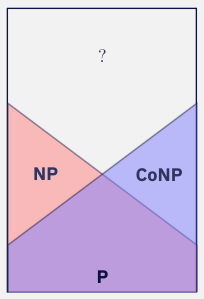
\includegraphics[width=0.7\linewidth]{images/basic-complexity-classes.png}
\end{wrapfigure}

Let $t:\mathbb{N} \to \mathbb{R}_{\geq 0}$. A time complexity class \textbf{TIME}$(t(n))$ is the collection of all problems that are decidable by a deterministic machine RM, TM etc.) in $\mathcal{O}(t(n))$ time.

Given $A = \{0^i1^i \:|\: i \in \mathbb{N}\}$, a TM can decide this in $\mathcal{O}(n^2)$, which means that $A \in$ \textbf{TIME}$(n^2)$.

We also define \textbf{NTIME}$(t(n))$ to be the collection of all problems decidable by a nondeterministic machine NRM, NTM, etc.) in $\mathcal{O}(t(n))$.
\end{dfn}

\begin{dfn}[P / Polynomial Time]{def:poly-time}{}
The polynomial complexity class \textbf{P} is the class of problems decidable with some deterministic polynomial time complexity.
\[\textbf{P} = \bigcup_{k \in \mathbb{N}} \textbf{TIME}(n^k)\]

Problems in \textbf{P} are called tractable. Any problem not in \textbf{P} is $\Omega(n^k)$ for every $k$.

The class itself is robust, reasonable changes to model don't change it and reasonable translations between problems preserves membership in \textbf{P}.

A polynomially-bounded RM together with a polynomial ($n^k$ for some $k$, without loss of generality), such that given an input $w$ it will always halt after executing $|w|^k$ instructions. A problem $Q$ is in \textbf{P} iff it is computed by such a machine.
\end{dfn}

\begin{dfn}[NP / Nondeterministic-polynomial time]{def:np-time}{}
The polynomial complexity class \textbf{NP} is the class of problems decidable with some nondeterministic polynomial time complexity.
\[\textbf{NP} = \bigcup_{k \in \mathbb{N}} \textbf{NTIME}(n^k)\]
\newline
We don't know if every exponentially bounded problem is in \textbf{NP}, we think that it's probably not the case.

\end{dfn}

\begin{dfn}[CoNP]{def:conp}{}
We don't know if the class NP is closed under complement. We cannot flip the result because the result of flipping in a nondeterministic machine involves turning it from angelic nondeterminism to demonic nondeterminism (otherwise known as co-nondeterminism) or vice versa.
\end{dfn}

\begin{dfn}[AP / Alternating Poly time]{def:AP}{}
The class \textbf{AP} is the class of all problems decidable by an alternating machine in polynomial time with no restriction on swapping quantifiers.

\textbf{AP} is known to be equal to PSPACE.
\end{dfn}

\begin{dfn}[PSPACE / Polynomial Space]{def:pspace}{}
An RM/TM is $f(n)$-space-bounded if it may use only $f(inputsize)$ space. For TMs this is the number of cells on the tape, where register machines uses bits in registers.

\end{dfn}

\begin{thm}[Polynomial Reductions]{thm:poly-reducts}{}
A polynomial reduction from $P_1 = (D_1, Q_1)$ to $P_2 = (D_2, Q_2)$ is a \textbf{P}-computable function $f : D_1 \to D_2$ such that $d \in Q_1$ iff $d \in Q_2$.

If $P_2$ is in \textbf{P}, then $P_1$ is in \textbf{P} straightforwardly. Therefore to prove a problem is not in \textbf{P} we can show that there is a polynomial reduction from a problem $P_2$ which isn't in \textbf{P} to our problem $P_1$

\renewcommand\labelitemi{\tiny$\bullet$}
\begin{itemize}
    \setlength\itemsep{0em}
    \item A problem $P_1$ is \textbf{polynomially reducible} to $P_2$, written $P_1 \leq_P P_2$ if there is a polynomially-bounded reduction from $P_1$ to $P_2$.
    \item A problem $P$ is \textbf{NP}-Hard if for every $A \in$ \textbf{NP}, $A \leq_P P$.
    
    That is, if a problem $P_1$ is \textbf{NP}-Hard and $P_1$ is polynomially reducible to $P_2$, then $P_2$ is also \textbf{NP}-Hard.
    
    We can use this fact to prove other problems are \textbf{NP}-Hard by showing a reduction from a known \textbf{NP}-hard problem.

    \item A problem is \textbf{NP}-Complete if it is both \textbf{NP}-Hard and in \textbf{NP}.

\end{itemize}

\end{thm}


\newpage

\begin{thm}[Cook-Levin Theorem]{thm:cook-levin}{}
The Cook-Levin theorem states that the NP problem SAT is NP-Complete.
\newline
The proof of this involves showing it is NP by nondeterministically guessing
assignments and checking them in polynomial time, and then showing it’s NP-
Hard by reducing any NP problem to SAT
\end{thm}


\subsection*{The Polynomial Heirarchy}
\begin{dfn}[Sigma Notation]{def:sigmas}{}
The set $\Sigma_{1}^{P}$ describes all problems that can be phrased as
\[\{y \mid \exists ^{p} x \in \mathbb{N} .\,R(x,y)\}\]
where $R$ is a \textbf{P}-decidable predicate and $\exists ^{p} x \dots$ indicates that $x$ is of size polynomial in the size of $y$.
\newline
We can say that $x$ is a certificate showing which guesses can be made by our NRM giving an accepting run.
\newline
If a problem $Q\in \Sigma^{P}_{1}$ then $Q$ is \textbf{NP}, because it is a problem for which we can verify the answer in polynomial time. If a problem $Q$ is in \textbf{NP} then $Q\in \Sigma^{P}_{1}$.
\newline
So, \textbf{NP} = $\Sigma^{P}_{1}$
\end{dfn}

\begin{dfn}[Pi notation]{def:pies}{}
The set $\Pi^{P}_{1}$ describes all problems that can be phrased as
\[\{y \mid \forall^{P}x \in \mathbb{N} . \, R(x,y)\}\]
where $R$ is a \textbf{P}-decidable predicate, and $\forall^{P}x\dots$ indicates that $x$ is of size polynomial in the size of $y$.
\newline
We have that
\[\Pi^{P}_{1} = \overline{\Sigma^{P}_{1}},\quad\text{and}\quad \Pi^{P}_{1} = \text{\textbf{CoNP}}\]
\end{dfn}

\begin{dfn}[Delta Notation]{def:deltas}{}
There are two conflicting definitions of $\Delta^{P}_{1}$ "For reasons that are unknown to me" - lecturer
\renewcommand\labelitemi{\tiny$\bullet$}
\begin{itemize}
    \setlength\itemsep{0em}
    \item The set $\Delta^{P}_{1}$ describes the intersection of $\Sigma^{P}_{1}$ and $\Pi^{P}_{1}$
    \item The set $\Delta^{P}_{1}$ describes the set \textbf{P}
\end{itemize}
From our characterisations of $\Sigma^{P}_{1}$ and $\Pi^{P}_{1}$, we have that $\Delta^{P}_{1}\subseteq \text{\textbf{P}}$, but we don't konw if these definitions are equal
\end{dfn}


\begin{dfn}[Moving higher]{def:next-dim-notations}{}
The next layer of the heirarchy goes as follows:
\begin{itemize}
    \item $\Sigma_2^P$ is all problems of the form $\{x \:|\: \exists^P y.\: \forall^P z.\: R(x,y,z)\}$
    \item $\Pi_2^P$ is all problems of the form $\{x \:|\: \forall^P y.\: \exists^P z.\: R(x,y,z)\}$
    \item $\Delta_2^P = \Sigma_2^P \cap \Pi_2^P$
\end{itemize}

\vspace{-5pt}
\noindent\rule{\textwidth}{0.2pt}
We can also use oracles to get an alternate definition:
\begin{itemize}
    \item $\Delta_2^P$ is all problems that are decidable in polynomial time by some deterministic RM/TM with an $\mathcal{O}(1)$ oracle for some problem in $\Sigma_1^P$ (it is \textbf{P} with an $\mathcal{O}(1)$ oracle for \textbf{NP})
    \item $\Sigma_2^P$ allows the TM/RM to be nondeterministic (it is \textbf{NP} with an $\mathcal{O}(1)$ oracle for \textbf{NP})
    \item $\Pi_2^P$ is \textbf{CoNP} with an oracle for \textbf{NP}
\end{itemize}

\vspace{-5pt}
\noindent\rule{\textwidth}{0.2pt}
In general for any $n>1$:
\begin{itemize}
    \item $\Delta_n^P$ is all problems decidable by a deterministic polynomially bounded TM/RM with an $\mathcal{O}(1)$ oracle for some problem in $\Sigma_{n-1}^P$.
    \item $\Sigma_n^P$ is all problems decidable by some nondeterministic polynomially bounded TM/RM with an $\mathcal{O}(1)$ oracle for some problem in $\Sigma_{n-1}^P$.
    \item $\Pi_n^P$ is all problems decidable by some co-nondeterministic polynomially bounded TM/RM with an $\mathcal{O}(1)$ oracle for some problem in $\Sigma_{n-1}^P$.
\end{itemize}
Note: Co-nondeterminism could also be called \textbf{demonic} nondeterminism, like regular (angelic) nondeterminism but only accepts if \textbf{all} paths accept
\end{dfn}


\begin{dfn}[Alternation]{def:alternation}{}
Equivalently $\Sigma^{P}_{n}$ are all problems that can be phrased as some \textbf{alternation} of (\textbf{P}-bounded) quantifiers, starting with $\exists^{P}$
\[\{ w \mid \exists^{P} x_{1} . \exists^{P} x_{2} . \exists^{P} x_{3} . \exists^{P} x_{4} . \dots x_{n} . R(w, x_{1}, \dots, x_{n})\}\]
$\Pi_n^P$ has a similar definition, starting instead with $\forall^P$
\[\{ w \mid \forall^{P} x_{1} . \exists^{P} x_{2} . \exists^{P} x_{3} . \exists^{P} x_{4} . \dots x_{n} . R(w, x_{1}, \dots, x_{n})\}\]

Alternating machines combine the acceptance modes of both angelic and demonic non-deterministic machines.

Alternating register machines would replace the NRM's \texttt{MAYBE} instruction with the \texttt{MAYBE}$^\exists$ and \texttt{MAYBE}$^\forall$ instructions, which are nondeterministic branching choices where acceptance depends on if one branch accepts ($\exists$) or both branches accept ($\forall$).

Alternating Turing Machines are defined by labelling states
with either $\forall$ or $\exists$.

The class $\Sigma_n^P$ can therefore be described as the class of problems decided in polynomial time by an alternating machine that initially uses $\exists$-nondeterminism and swaps quantifiers at most $n-1$ times. This extends to $\Pi_n^P$ swapping starting with $\exists$ to starting with $\forall$.
\end{dfn}

blank filler text: \lipsum[1-12]


% This is what a boxed environment is formatted like
% Different formats are:
    % dfn : definition
    % thm : theorem
    % xmp : example
    % rem : remark

% First field is name - that's what shows up on the paper
% Second field is just to reference, not too important
% Leave the last field blank, it was lecture note numbers from FPM and
% but atm i cba changing the environment doesn't look the prettiest but o well
\begin{dfn}[Name]{def:Label}{}

\end{dfn}

\newpage
\begin{xmp}[Regular Expressions]{def:ex-regex}{}
At least one $0$:
\[(0\cup 1) ^{*} 0(0\cup 1)*\]
At least one $1$ and at least one $0$:
\[((0 \cup 1)^*01(0 \cup 1)^*) \cup ((0 \cup 1)^*10(0 \cup 1)^*)\]
\end{xmp}

\end{multicols}

\end{document}